\section{Auswertung}
\label{sec:Auswertung}
\subsection{Berechnung der Aktivierungsarbeit aus der Anlaufkurve}
Um die Aktivierungsarbeit der Dipole zu berechnen, werden die Messwerte für Temperatur und Strom
mit der Exponentialfunktion der Form
\begin{equation}
  y(T) = a\cdot e^{mT}
  \label{eqn:efit}
\end{equation}
gefittet.
% Mittlere heizspannung efit 3.2 0.13
\begin{figure}[H]
  \centering
  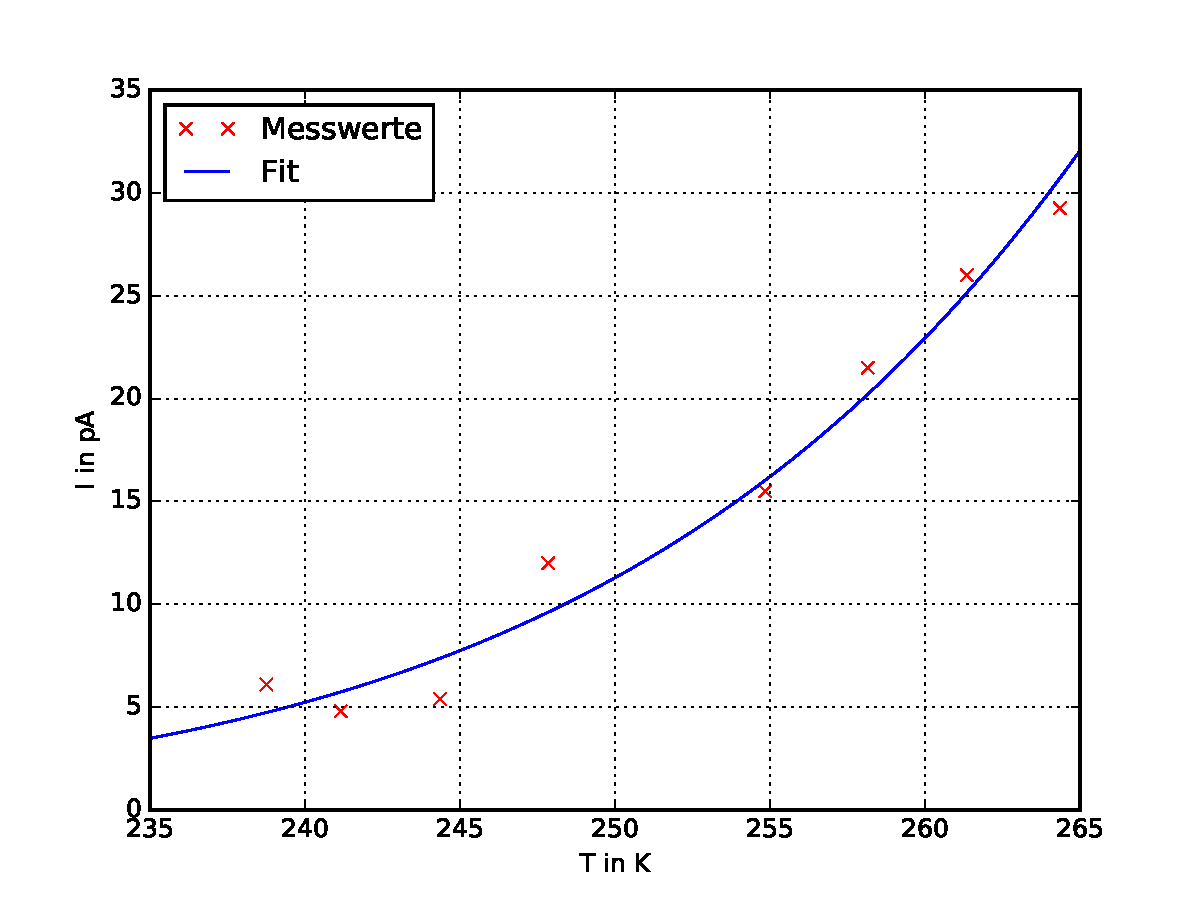
\includegraphics[width=0.8\textwidth]{plots/efit.pdf}
  \caption{Anlaufkurve des Depolarisationsstromes bei einer mittleren Heizrate von $H_1 =\SI{3.3 \pm 0.08}{\kelvin\per\minute}$.}
  \label{fig:efit1}
\end{figure}
\begin{figure}[H]
  \centering
  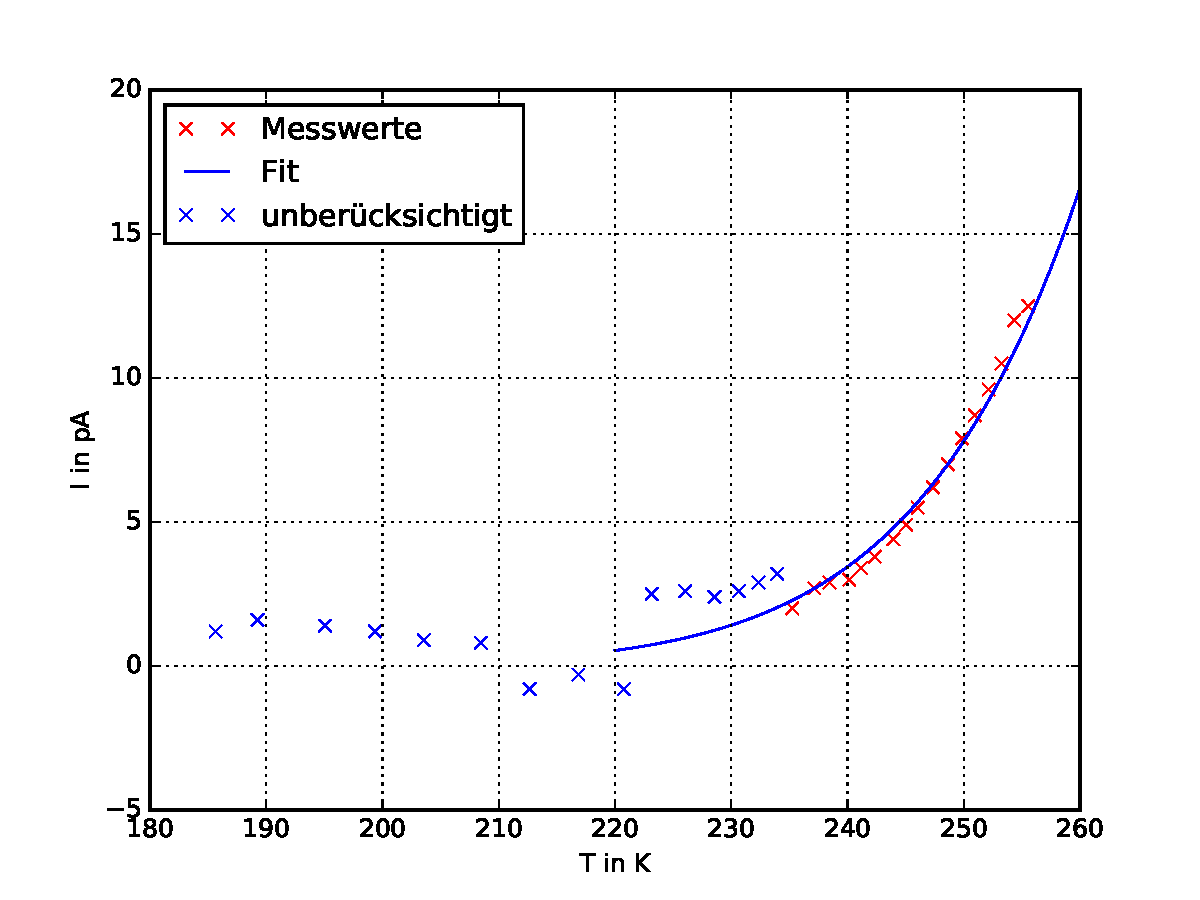
\includegraphics[width=0.8\textwidth]{plots/efit2.pdf}
  \caption{Anlaufkurve des Depolarisationsstromes bei einer mittleren Heizrate von $H_2 =\SI{1.26 \pm 0.07 }{\kelvin\per\minute}$}
  \label{fig:efit2}
\end{figure}
Die gefitteten Anlaufkurven sind in Abbildung \ref{fig:efit1} und \ref{fig:efit2} zu sehen.
Für den Fit der zweiten Messung wurden die in Abbildung \ref{fig:efit2} gezeigten bauen Messwerte nicht berücksichtigt.
Aus den angehängten Messwerten wurden ausserdem mittlere Heizraten für beide Messungen bestimmt. Die aus den Werten der Anlaufkurve ermittelten Heizraten lauten:
\begin{center}
  $H_1 =(3.2 \pm 0.13)\frac{\symup{K}}{\text{min}}$, $H_2 = (1.26 \pm 0.064)\frac{\symup{K}}{\text{min}}$
\end{center}
Aus der Ausgleichsrechnung ergeben sich die Fitparameter zu
\begin{center}
    $m_1 = 5680.23$, $ a_1= 24.98$, $m_2 = 5425.56$, $a_2 = 23.87$.
\end{center}
Aus dem Fitparameter $m_{(1/2)}$ werden dann nach
\begin{equation}
  W_{1/2} = m_{1/2}\cdot k_B
\end{equation}
die Austrittsarbeiten berechnet. Die berechneten Arbeiten lauten:
\begin{center}
  $W_1 = \SI{0.78e-19}{\joule}$ und $W_2 = \SI{0.75e-19}{\joule}$
\end{center}
\subsection{Berechnung der Aktivierungsenergie durch Integrieren}

Die mittleren Relaxationszeiten der Probe wurden durch \eqref{eqn:tau2} unter Zuhilfenahme riemannscher Integration berechnet und in Abb. \ref{fig:integral} dargestellt. Hierbei wurde der zweite Anstieg jeweils nicht betrachtet.

\begin{figure}
  \centering
  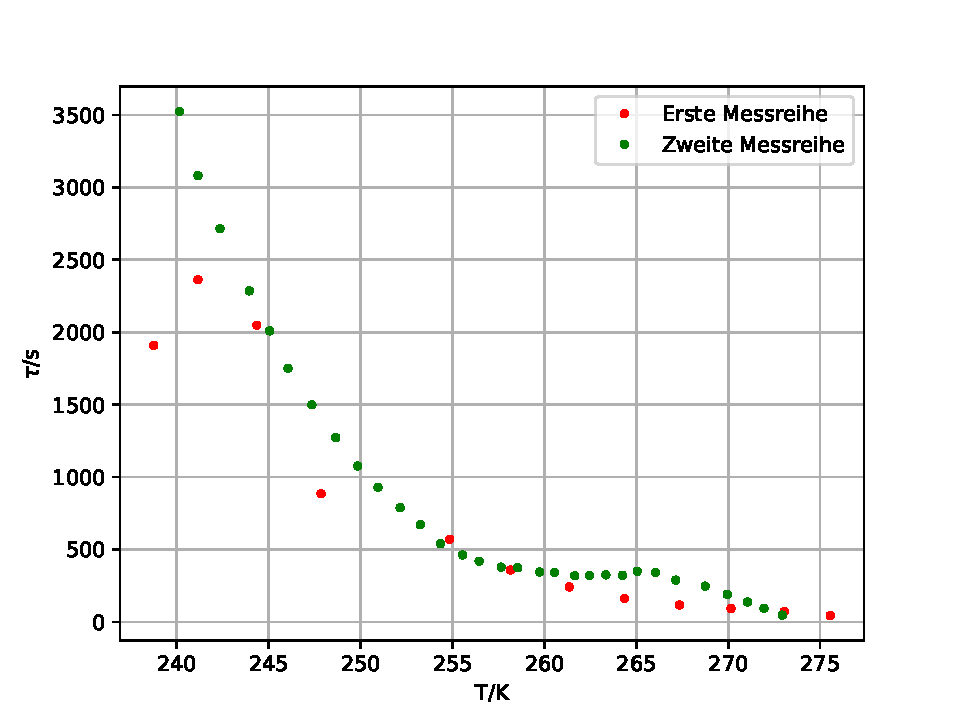
\includegraphics{./plots/integral.pdf}
  \caption{Mittlere Lebensdauern $\tau(T)$ der Probe in Abhängigkeit der Temperatur $T$.}
  \label{fig:integral}
\end{figure}

Eine lineare Ausgleichsrechnung von $\ln(\tau(T)\cdot H)$ augetragen gegen $1/T$ (siehe Abb. \ref{fig:log}) liefert
\begin{center}
  $m_1 = \SI{7417 \pm 426}{\kelvin}$ und $b_1 = -25.5\pm1.6$
\end{center}
für die erste Messung. $m$ bezeichnet hierbei die Steigung der Geraden, $b$ den Ordonatenabschnitt.
Es ergibt sich hierdurch
\begin{equation*}
  W_1^i = k_b m_1 = \SI{102 \pm 6}{\zepto\joule}.
\end{equation*}

\begin{figure}
  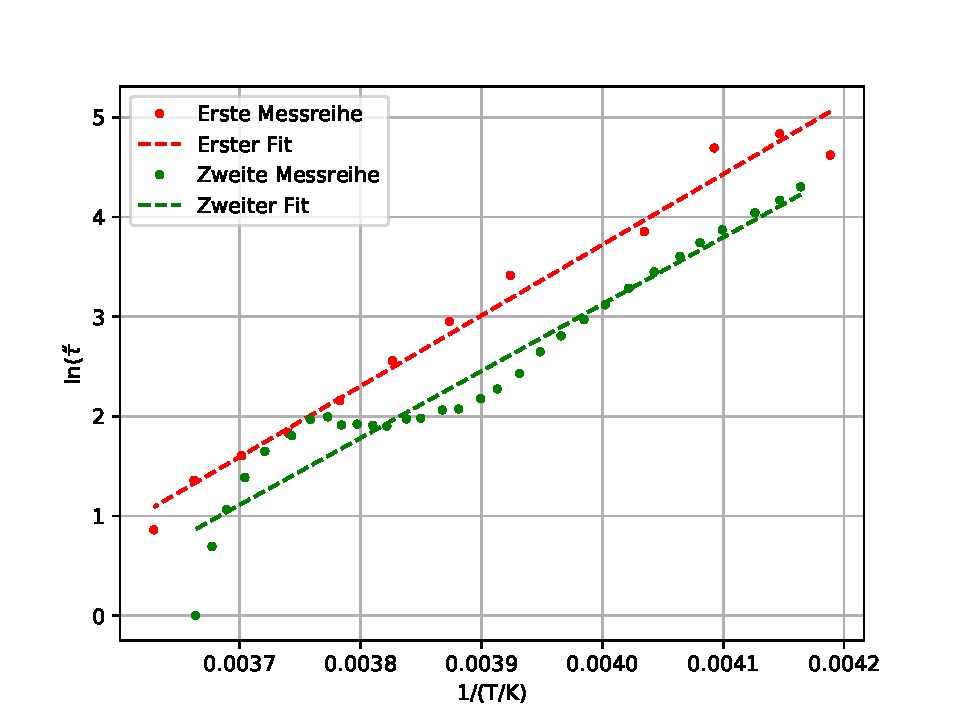
\includegraphics{./plots/log.pdf}
  \caption{}
  \label{fig:log}
\end{figure}

Für die zweite Messreihe ergibt sich entsprechend:
\begin{center}
  $m_2 =  \SI{6713 \pm 324}{\kelvin}$, $b_2=-23.7 \pm 1.3$, $W_2^i= \SI{93 \pm 4}{\zepto\joule}$
\end{center}

\subsection{Bestimmung der charakteristischen Relaxationszeit}
Als Maxima wurden gewählt:
\begin{center}
  $T_{max,1} = \SI{-8.8}{\celsius}$ und $T_{max,2} = \SI{-16.7}{\celsius}$
\end{center}
Nach Verrechnung dieser Werte, sowie $W_1$ bzw. $W_2$, ergibt sich gemäß \eqref{eqn:tau3}:
\begin{center}
  $\tau_{max,1}=  \SI{177\pm 10}{\second}$ und $\tau_{max,2}=  \SI{466\pm23}{\second}$
\end{center}

Dieser Werte lassen sich wiederrum durch \eqref{eqn:relaxation} in $\tau_0$ überführen.
Dies liefert
\begin{center}
  $\tau_{0,1}= \SI{0.12 \pm 0.19}{\nano\second}$ und $\tau_{0,2} = \SI{2.0 \pm 2.6}{\nano\second}$.
\end{center}
